\documentclass{article}
\usepackage[utf8]{inputenc}
\usepackage{cite}
\usepackage{amsmath}
\usepackage{amssymb}
\usepackage{pgfplots}
\usepackage{filecontents}
\usepackage{verbatim}
\usepackage[]{algorithm2e}

\usepackage{placeins}
\let\Oldsection\section
\renewcommand{\section}{\FloatBarrier\Oldsection}
\let\Oldsubsection\subsection
\renewcommand{\subsection}{\FloatBarrier\Oldsubsection}
\let\Oldsubsubsection\subsubsection
\renewcommand{\subsubsection}{\FloatBarrier\Oldsubsubsection}

%\usepackage{unicode-math}

\usepgfplotslibrary{external} \tikzexternalize
%\usetikzlibrary{pgfplots.external}

\title{COMP4620 Assignment 2}
\author{Joseph Meltzer, Xi Du, Tianyu Wang, Xavier O'Rourke}
\date{October 2018}

\begin{document}


\maketitle
\begin{flushleft}

%\section{Using the agent} 

%To compile the agent run \texttt{make main} in terminal. To run the agent, enter \texttt{./agent <environment\_name>.conf} where \texttt{<environment\_name>} is an environment from the following list:
%\begin{itemize}
%    \item coinflip
%    \item tictactoe
%    \item rps
%    \item 1dmzae
%    \item cheezemaze
%    \item pacman
%\end{itemize}

\section{Agent Implementation}

\subsection{Context Tree Weighting}



The code which implements the Context Tree Weighting algorithm may be found in the \texttt{predict.cpp} and \texttt{predict.hpp} files. The implementation is commensurate with the provided interfaces. The implementation uses a tree data-structure composed of several \texttt{CTNode} objects. Each \texttt{CTNode} encapsulates data about the number of $0$s and $1$s we have seen in that node's context, the value of the log of the KT estimator at that node, as well as the log of the weighted probability at that node (referred to as $P^n _w$ in \cite{orig}), as well as pointers to that node's children. \newline

The most difficult part of this module's implementation was the \texttt{ContextTree::Update} and \texttt{ContextTree::Revert} methods. When we want to update our tree with a new symbol, this means updating the symbol counts, KT estimators and weighted probabilities of the node corresponding to this context, as well as all ancestors of that node. This is achieved by first following a path down from the root node of the tree to the bottom (checking the previous symbol in the history at every step to decide which branch to traverse) while updating the symbol counts. Once we reach a leaf node at maximum depth, we then retrace our steps moving back up the tree while updating the probability estimates. \newline

When we update the weighted probability estimates we use equation (27) in \cite{orig}, which defines the weighted estimates as follows

  \[
    P_w ^n := \left\{\begin{array}{lr}
        Pr_{kt}(h_{T, n}), & \textrm{if } n \textrm{ is a leaf node.}\\
        \frac{1}{2}Pr_{kt}(h_{T, n}) + \frac{1}{2}P^{n0}_w \times P^{n1}_w & \textrm{otherwise } \\
        \end{array}\right\}
  \]
In our original implementation we calculated this estimate by naively evaluating the expression

\[
    \log P_w^n = \log \bigg( 0.5 \times \exp x + 0.5 \times \exp ( y \times z) ) \bigg)
\]

Where $x = \log (Pr_{kt}(h_{T, n}))$, $y = \log P^{n0}_w$, and $z = \log P^{n1}_w$. \newline

This implementation resulted in erratic agent behaviour when the size of the agent's history grew large. The problem here is that when the history is long, our probability estimates become extremely close to zero, meaning we take the log of a very small number, which can lead to underflow. To correct this, we borrowed a trick from the original implementation and calculated our log weighted probability estimates according to the equivalent formula:

$$
    \log P_w^n = \log 0.5 + a + \log (1 + e^{b - a})
$$

Where \begin{align*}
    a =  \max&\{ \log Pr_{kt}(h_{T, n}), \log (P^{n0}_w \times P^{n1}_w) \} \\
    b =  \min&\{ \log Pr_{kt}(h_{T, n}), \log (P^{n0}_w \times P^{n1}_w) \}
\end{align*}

Our CTW algorithm makes predictions about the next bit in our history $h$ using the law of conditional probability: 

\[
    \mathbb{P}(0 | h) = \dfrac{\mathbb{P}(h0)}{\mathbb{P}(h)} \qquad \mathbb{P}(1 | h) = 1 - \dfrac{\mathbb{P}(h0)}{\mathbb{P}(h)}
\]

This means, when calling \texttt{ContexTree::genRandomSymbolsAndUpdate()} or \texttt{ContexTree::predict()} we need to update the tree \textit{as if} we have just observed a $0$, and compare the estimated likelihood of the old history to the new history to determine with what probability we should predict the next bit to be a $0$. \newline

% The CTW code was written by Xavier. Tianyu and Xi assisted with testing the implementation and identifying bugs.

\subsection{Monte Carlo Search Tree}

The code which implements the Monte Carlo Search Tree may be found in the search.cpp and search.hpp files. \newline

The tree structure is implemented as follows. 
As provided in the interface, each node is a SearchNode class. The edges between nodes are implemented with C++ map object, which is a member of the parent node, containing pointers pointing to its child nodes. C++ map is essentially a red-black tree which allows insert and find objects according to keys in $O(\log n)$ time. In our implementation, the keys stored in an action node (the keys of all the child nodes of the action node) is the decoded binary representation of the actions. The key stored in an chance node (the keys of all the child nodes of the chance node) is the decoded concatenated binary representation of both observation and reward. Observation is appended to the end of the reward.\newline

The sampling process is an implementation of Algorithm 1,2,3,4 in [1]. A random ties breaker of incremental fashion is used when multiple max values can be found. For a list $\mathbf{v}$, the elements of which are real values, the largest value can be selected through one iteration of $\mathbf{v}$ without knowing the length of $\mathbf{v}$ or the number of elements that have the largest value. The detailed ties breaker is as follows.

\begin{algorithm}[H]
 \KwData{$\mathbf{v}$,  $num\_ties = 1$, $v\_max = -\infty$}
 \KwResult{Select the element with largest value with uniformly random ties breaker}

 \For{$v$ in $\mathbf{v}$}
 {
  \uIf{$v > v\_max$}
  {
   $v\_max = v$\;
   $num\_ties = 1$;
  }
  \uElseIf{$v\_max == v$}
  {
    $v\_max = v$ with probability $1 - \frac{num\_ties}{num\_ties + 1}$ \;
    $num\_ties = num\_ties + 1$;
  }
 }
 \caption{Ties Breaker}
\end{algorithm}

Assume that there are in total $n$ elements have the max value $x$.
According to this algorithm, the probability that one element is selected is $\frac{1}{n}$ for all $n$ elements. Thus, we achieved a strict uniformaly random ties breaker. \newline

In order to debug the MCST, we also added interface to let the AIXI directly samples from the true environments during the role out. \newline

% The MCST code was written by Tianyu. Xavier and Xi assisted with testing the implementation and identifying bugs.\newline


\section{Implemented Environments}

\textbf{CoinFlip } This is just the CoinFlip example in the provided template. 
The value for the \verb|environment| option is \verb|coin-flip|.
\newline

\textbf{1d-Maze. } The 1d-maze has been implemented as specified in the assignment specification. The length of the maze is configurable and so is the position of the goal/reward location within the maze. The environment will continue to run even after the agent has reached the goal once. 

The value for the \verb|environment| option is \verb|1d-maze|.
\newline

\textbf{Cheese Maze. } This domain has been implemented as per the specification, with modifications to the reward values. The rewards have been scaled to non-negative integers as follows: Bumping into a wall rewards 0. Moving into a free cell that does not have the cheese rewards 9, and finding the cheese rewards 20. Again, the agent finding the cheese does not reset or stop the the environment. 

The value for the \verb|environment| option is \verb|cheese-maze|.
\newline

\textbf{TicTacToe. } TicTacToe is implemented with an opponent (the environment) which makes random moves as per the specification. The rewards have been scaled to be non-negative as follows: Making an illegal move rewards 0. Losing to the environment rewards 1. Making a legal but not game-ending move rewards 2. Ending the game with a draw rewards 3, and winning rewards 4. The games of TicTacToe are repeated, with a new game starting as soon as the previous is completed. 

The value for the \verb|environment| option is \verb|tictactoe|.
\newline

\textbf{Biased Rock-Paper-Scissors. } Rock-Paper-Scissors is implemented with the opponent bias as specified. The rewards are scaled such that 0 is a loss, 1 is a draw and 2 is a win. 

The value for the \verb|environment| option is \verb|biased-rock-paper-scissor|.
\newline

\textbf{PacMan. } 
This version of the PacMan was implemented with the 
effort to minimise the number of states remaining across cycles.
As a by-product, the resulting code is less than 400 lines long,
complete with power pill effect and comments.
It were implemented to meet the requirements, including follow-up
ones from communications, as closely as possible.
The relevant words from the requirements are placed 
in the source code as comments enclosed in quotation marks,
alongside corresponding implementations.
The rewards were shifted with 128 but in this report they
were shifted back.

Most importantly, we ended up programming a visualisation tool 
to detect bugs, although not required.
The visualisation simply prints the game screen as 
ASCII characters to \verb|stdout|. Because the output
quickly fills up the console, the latest game screen
will always on the bottom, effectively becoming animation
if you stare at it, and the program is not running too
fast (which true for meaning for simultaions).
The visualisation is hardcoded and cannot be disabled,
unless commented out in the source.
During experimenting we mostly piped the \verb|stdout|
to a \verb|.txt|file. In this case,
running in Linux shell
\begin{verbatim}
tail -f <the output file containing stdout>
\end{verbatim}
would then print the game in realtime.
Actually it looked better with \verb|tail -f|
because of output buffering, hence showing no "stream
of lines" but whole blocks at once.


The value for the \verb|environment| option is \verb|pacman|
\newline

\section{Usage and Testing}

\subsection{Basic usage}
The way to compile and run the code is largely unchanged from that in the assignment requirement.
Assuming the necessary POSIX tools, to compile, \verb|cd| into the source tree and 
run 
\begin{verbatim}
make main
\end{verbatim}
To execute the binary, run
\begin{verbatim}
./main coinflips.conf logfile
\end{verbatim}
where the semantics of the arguments are exactly the same as in the requirement.


\subsection{Test harness}

A minimalist test harness, complete with parallel execution, was implemented with 
a single line of Bash script in \verb|streambatch.sh|.
%\verbatiminput{streambatch.sh}

There are a few precautions before use.
All \verb|.conf| files of interest need to be under \verb|cf/|.
There needs to be a writable directory \verb|logs/|, under which
are corresponding sub-directories if \verb|.conf| files are in 
sub-directories of \verb|cf/|. The script does not create
directories on its own.

For example, if we are to test \verb|cf/abc/123.conf|, there has to be
a directory \verb|logs/abc/| for the script to work.

Then we simply pipe into the \verb|stdin| of \verb|streambatch.sh| the paths of 
\verb|.conf| files to be tested, one line each.

For example, to test all \verb|cf/short/*-coinflip.conf| files, 
run 
\begin{verbatim}
ls cf/short/*-coinflip.conf | bash streambatch.sh
\end{verbatim}
and then the outputs will be written to \verb|cf/short/*-coinflip.txt|,
\verb|cf/short/*-coinflip.log| and
\verb|cf/short/*-coinflip.csv|.
The \verb|.txt| files are for the human-readable output, while \verb|.log| and
\verb|.csv| being the longer, detailed logs as specified in the assignment
requirement.
If there are errors or warnings, they will be in the \verb|.err| files.

At most 6 jobs by default will be run in parallel, which is suitable for most desktop
computers.

\subsection{Post-processing}
To keep the reward values nonnegative, some of the environments have their rewards
translated.
However, the reward of the first cycle was always zero and
thus rendered the figure of average rewards less informative.
To compensate this without re-running all the experiments,
the plots in this report use recalculated
\begin{align*}
\frac{\text{total reward}}{\text{cycle} - 1}
\end{align*}
as the average reward.

%\begin{tikzpicture}[trim axis left]
%\begin{axis}[legend pos = south east, width=\textwidth, height=0.5\textwidth]
%\addplot [orange,no marks] table [x=cycle, y=average reward, col sep=comma] {95d-coinflip.csv};
%\addlegendentry{0.95 Decay}
%\addplot [cyan,no marks] table [x=cycle, y=average reward, col sep=comma] {o-coinflip.csv};
%\addlegendentry{Fully Exploit}
%\end{axis}
%\end{tikzpicture}

\newcommand{\one}[1]{
\addplot table [x=cycle, y expr=\thisrow{total reward}/(\thisrow{cycle}-1), col sep=comma] {#1};
}

\newcommand{\avg}[1]{
\addplot table [x=cycle, y expr=\thisrow{winavg}, col sep=comma] {#1};
}


\newcommand{\five}[1]{
\one{../logs/short/o-#1.csv}
\addlegendentry{Always Exploit}
\one{../logs/short/r-#1.csv}
\addlegendentry{Always Random}
\one{../logs/short/0.1-#1.csv}
\addlegendentry{0.1 Explore}
\one{../logs/short/95d-#1.csv}
\addlegendentry{0.95 Decay}
\one{../logs/short/p-#1.csv}
\addlegendentry{Real Env}
}

\def \stdAO {
legend pos = south east, 
cycle list={cyan,magenta,teal,orange,violet,brown,black,pink,yellow,lime,red,green,blue,olive,purple,black!50!white},
width=40em, %\expandafter{\textwidth}, 
height=20em,
no marks
}

\def \stdAOM {
legend pos = outer north east, 
cycle list={cyan,magenta,teal,orange,violet,brown,black,pink,yellow,lime,red,green,blue,olive,purple,black!50!white},
width=34em, %\expandafter{\textwidth}, 
height=20em,
no marks
}

\newcommand{\cpt}[1]{
\caption{Average reward vs. time for #1}
}

\section{Results}

\subsection{CoinFlip}

For the CoinFlip we initially considered five standard 
configurations with
\begin{verbatim}
ct-depth = 4
agent-horizon = 2
\end{verbatim}
and a head-probability of $0.1$.

The first configuration “Always Exploit”
has \verb|exploration| set to $0$
to keep the agent from exploring at all.

The second configuration “Always Random”
has both \verb|exploration|
and \verb|explore-decay| set to $1$
to imitate pure random play.

The third and fourth configurations “0.1 Explore”
and “0.95 Decay”
represent two strategies of mixing exploration and
exploitation, with
\begin{verbatim}
exploration = 0.1
explore-decay = 1
\end{verbatim}
and
\begin{verbatim}
exploration = 1
explore-decay=0.95
\end{verbatim}
respectively.

The last configuration “Real Env” 
is configured to always exploit and use
an authentic \verb|Environment| as 
an “oracle” to do
the prediction.
Note that the oracle does not tell 
the agent what the next toss will
be head or tail, but instead toss a coin
with the true probability ($0.1$),
which is independent from the
"real" toss in the next cycle.

Then we tested a final configuration specific
to the CoinFlip environment,
which always exploits with 
\begin{verbatim}
ct-depth = 0
agent-horizon = 0
\end{verbatim}

\begin{figure}
\begin{tikzpicture}[trim axis left]
\begin{axis}[ \stdAO , skip coords between index={0}{1}]
\five{coinflip}
\one{../logs/sp1-coinflip.csv}
\addlegendentry{D=0 H=0}
\end{axis}
\end{tikzpicture}

\begin{tikzpicture}[trim axis left]
\begin{semilogxaxis}[ \stdAO , skip coords between index={0}{20}]
\five{coinflip}
\one{../logs/sp1-coinflip.csv}
\addlegendentry{D=0 H=0}
\end{semilogxaxis}
\end{tikzpicture}
\cpt{\label{fig:cf} CoinFlip}
\end{figure}

In Figure \ref{fig:cf}, we first display the
average reward with respect to time.

To show the initial process of learning more clearly, a log-time plot with
first 20 cycles removed (to cancel the fluctuation of average heads initially) will be displayed next.

We can see that the average reward of pure random playing converges
to 0.5, and other strategies converge to higher values as expected.

However, we also found that search trees 
with "more than enough" capabilities actually worsen the
performance. Only in the "D=0 H=0" configuration,the agent 
learnt to deterministically guess
tail, which is the optimal strategy, and achieved an average reward of $0.9$.

Otherwise, even with exploration turned off and true probabilities given,
the agent tend to randomly guess with the $0.9$ chance of tail and ends up with
an average reward of around $0.8$.

\newpage

\subsection{1d-Maze}

First we tried the aforementioned five standard tests
in the 1d-Maze environment, results shown in Figure \ref{fig:1d}
We can see that a fully random strategy converges to
an average reward of around $0.25$.
The long-period oscillation of the other strategies
hint a lack of memory.
Constant exploration seems to be able to break this
oscillation though, at the cost of peak performance.

\begin{figure}
\vspace{-30em}
\begin{tikzpicture}[trim axis left]
\begin{axis}[ \stdAO , skip coords between index={0}{1}]
\five{1dmaze}
\end{axis}
\end{tikzpicture}

\begin{tikzpicture}[trim axis left]
\begin{semilogxaxis}[ \stdAO , skip coords between index={0}{20}]
\five{1dmaze}
\end{semilogxaxis}
\end{tikzpicture}
\cpt{\label{fig:1d} 1d-Maze}
\end{figure}

\newpage

\begin{figure}
\vspace{-5em}
\begin{tikzpicture}[trim axis left]
\begin{axis}[ \stdAO , skip coords between index={0}{10}]
\one{../logs/shorter-8/95d-1dmaze.csv}
\addlegendentry{D=8 H=3}
\one{../logs/shorter-16/95d-1dmaze.csv}
\addlegendentry{D=16 H=4}
\one{../logs/shorter-32/95d-1dmaze.csv}
\addlegendentry{D=32 H=5}
\one{../logs/shorter-64/95d-1dmaze.csv}
\addlegendentry{D=64 H=6}
\one{../logs/shorter-128/95d-1dmaze.csv}
\addlegendentry{D=128 H=7}
\one{../logs/shorter-256/95d-1dmaze.csv}
\addlegendentry{D=256 H=8}
\one{../logs/shorter-512/95d-1dmaze.csv}
\addlegendentry{D=512 H=9}
\end{axis}
\end{tikzpicture}
\cpt{\label{fig:1d2} 1d-Maze of Various (D,H)}
\end{figure}

Then we ran multiple tests with 0.95 decay but different tree depths and 
agent horizons, results shown in Figure \ref{fig:1d2}.
The optimal strategy would be to keep moving away from 
and then moving back to the target cell,
with an average reward of $0.5$.
In this case all configurations seemed to converge to this maximum of $0.5$,
even with "more than enough" depth and horizon,
different from that in CoinFlip.

Best results with more cycles are shown in Figure \ref{fig:1d3} along with log-time graph.

\newpage

\begin{figure}
\begin{tikzpicture}[trim axis left]
\begin{axis}[ \stdAO , skip coords between index={0}{1}]
\one{../logs/sp1-1dmaze.csv}
\addlegendentry{D=32 H=5}
\one{../logs/sp2-1dmaze.csv}
\addlegendentry{D=8 H=3}
\end{axis}
\end{tikzpicture}

\begin{tikzpicture}[trim axis left]
\begin{semilogxaxis}[ \stdAO , skip coords between index={0}{100}]
\one{../logs/sp1-1dmaze.csv}
\addlegendentry{D=32 H=5}
\one{../logs/sp2-1dmaze.csv}
\addlegendentry{D=8 H=3}
\end{semilogxaxis}
\end{tikzpicture}
\cpt{\label{fig:1d3} 1d-Maze}
\end{figure}

\newpage

\subsection{Cheese Maze}

As usual we tried the five standard tests
in the Cheese Maze environment, results shown in Figure \ref{fig:cm}
We can see that a fully random strategy converges to
an average reward of around $4.2$.
The advantages optimized agents have over a purely random agent
is marginal, suggesting that we increase the tree depth
and search horizon.
Although the optimal strategy of this game is simply
moving away from and then back to the cheese,
The agent has to decide whether it is in 
the second column from history due to the perceptual aliasing.

\begin{figure}
\vspace{-30em}
\begin{tikzpicture}[trim axis left]
\begin{axis}[ \stdAO , skip coords between index={0}{1},
each nth point = 50,
filter discard warning=false
]
\five{cheesemaze}
\end{axis}
\end{tikzpicture}

\begin{tikzpicture}[trim axis left]
\begin{semilogxaxis}[ \stdAO , skip coords between index={0}{100},
each nth point = 50,
filter discard warning=false
]
\five{cheesemaze}
\end{semilogxaxis}
\end{tikzpicture}
\cpt{\label{fig:cm} Cheese Maze}
\end{figure}

\newpage

Then we tested several configuration sizes, with 
horizon and tree depth scaling together, 
as shown in Figure \ref{fig:cm2}.

\begin{figure}
\begin{tikzpicture}[trim axis left]
\begin{axis}[ \stdAO , skip coords between index={0}{10},
each nth point = 10,
filter discard warning=false
]
\one{../logs/shorter-8/95d-cheesemaze.csv} \addlegendentry{D=8 H=3}
\one{../logs/shorter-16/95d-cheesemaze.csv} \addlegendentry{D=16 H=4}
\one{../logs/shorter-32/95d-cheesemaze.csv} \addlegendentry{D=32 H=5}
\one{../logs/shorter-64/95d-cheesemaze.csv} \addlegendentry{D=64 H=6}
\one{../logs/shorter-128/95d-cheesemaze.csv} \addlegendentry{D=128 H=7}
\one{../logs/shorter-256/95d-cheesemaze.csv} \addlegendentry{D=256 H=8}
\one{../logs/shorter-512/95d-cheesemaze.csv} \addlegendentry{D=512 H=9}
\end{axis}
\end{tikzpicture}
\cpt{\label{fig:cm2} Cheese Maze}
\end{figure}

It seems like the models are not the larger
the better. More extensive tests resulted
in what is displayed in Figure \ref{fig:cm3}.

While we did not run the experiments until the
average rewards visually moved to the optimal value 
$14.5$ by moving
back and forth onto the cheese position and receiving
(shifted) rewards of $9$ and $20$ alternatively,
manual inspection of the logfiles revealed
that agents with the first four configurations
did converge to this behaviour.
The case “D=16 H=4 R” was configured to use
the real environment for prediction, which did
not show good results in this case.
In the corner case with zero agent horizon,
the agent ended up keep running into walls.

The conclusion we draw is that there is a
hard minimum of tree depth, greater than 16 
and less or equal to 32, with which the
agent can converge to an optimal behaviour,
although we didn't actually pin down this limit
due to limited computational resource.
More than that, deeper trees might make learning faster 
(in terms of cycles). 
The search horizon must be at least 1, 
best to be 2, but past that point, larger horizons quickly
deteriorate learning rate.

\def\cmcurves{
%\one{../logs/spE-cm.csv} \addlegendentry{D=8 H=2}
%\one{../logs/spE-p-cm.csv} \addlegendentry{D=8 H=2 R}
\one{../logs/sp4-cheesemaze.csv} \addlegendentry{D=64 H=2}
\one{../logs/sp6-cheesemaze.csv} \addlegendentry{D=32 H=2}
\one{../logs/sp9-cheesemaze.csv} \addlegendentry{D=64 H=1}
\one{../logs/sp7-cheesemaze.csv} \addlegendentry{D=32 H=1}
\one{../logs/spD-cm.csv} \addlegendentry{D=64 H=3}
\one{../logs/spC-cm.csv} \addlegendentry{D=32 H=3}
\one{../logs/sp2-cheesemaze.csv} \addlegendentry{D=32 H=4}
\one{../logs/sp5-cheesemaze.csv} \addlegendentry{D=64 H=4}
\one{../logs/spA-cm.csv} \addlegendentry{D=16 H=2}
\one{../logs/sp1-p-cheesemaze.csv} \addlegendentry{D=16 H=4 R}
\one{../logs/spB-cm.csv} \addlegendentry{D=16 H=3}
\one{../logs/sp1-cheesemaze.csv} \addlegendentry{D=16 H=4}
%\one{../logs/sp3-cheesemaze.csv} \addlegendentry{D=2 H=2}
\one{../logs/sp8-cheesemaze.csv} \addlegendentry{D=32 H=0}
}

\begin{figure}
\begin{tikzpicture}[trim axis left]
\begin{axis}[ \stdAOM , skip coords between index={0}{10}, 
each nth point = 60,
filter discard warning=false
] \cmcurves
\end{axis}
\end{tikzpicture}

\begin{tikzpicture}[trim axis left]
\begin{semilogxaxis}[ \stdAOM , skip coords between index={0}{10}, 
each nth point = 20,
filter discard warning=false
] \cmcurves
\end{semilogxaxis}
\end{tikzpicture}
\cpt{\label{fig:cm3} Cheese Maze}
\end{figure}

\newpage
\subsection{Biased Rock-Paper-Scissors}

As usual we did the five standard tests to get a basic idea from Figure
\ref{fig:rps}.
Again we found the default model too small and the advantages marginal.

Luckily, this game was quick to simulate and did not require a complex model
to play since there are only 3 possible actions and it is a 1D Markov 
process. So we were able to do extensive tests on this game, results shown 
in Figure \ref{fig:rps}.

Only with tree depth of 16 and agent horizon of 2 did the 
agent converge to the optimal value of 1.2.
It looks like with D=12 H=1 or D16 H1 it could converge
to 1.2 as well, but we anticipated the simulation to be
of too many cycles to to carry.

In general, learning the Biasd Rock-Paper-Scissors seems
to be a slow task for hour agent, while the game it self being simple. 
The optimal agent horizon appears to vary with the tree depth, 
unlike that in the Cheese Maze problem.

\begin{figure}
\vspace{-30em}
\begin{tikzpicture}[trim axis left]
\begin{axis}[ \stdAO , skip coords between index={0}{1}]
\five{rps}
\end{axis}
\end{tikzpicture}

\begin{tikzpicture}[trim axis left]
\begin{semilogxaxis}[ \stdAO , skip coords between index={0}{30}]
\five{rps}
\end{semilogxaxis}
\end{tikzpicture}
\cpt{\label{fig:rps} Biased Rock-Paper-Scissors}
\end{figure}

\def\rpscurves*{
\one{sp7-rps.csv}   \addlegendentry{D=16 H=2}
\one{spA-rps.csv}   \addlegendentry{D=12 H=1}
\one{spE-rps.csv}   \addlegendentry{D=10 H=1}
\one{spD-rps.csv}   \addlegendentry{D=10 H=2}
\one{sp1-rps.csv}   \addlegendentry{D=12 H=2}
\one{sp1-p-rps.csv} \addlegendentry{D=12 H=2 R}
\one{sp3-rps.csv}   \addlegendentry{D=6 H=2}
\one{sp2-p-rps.csv} \addlegendentry{D=4 H=2 R}
\one{sp4-rps.csv}   \addlegendentry{D=4 H=4}
\one{sp2-rps.csv}   \addlegendentry{D=4 H=2}
\one{sp9-rps.csv}   \addlegendentry{D=12 H=2}
\one{sp6-rps.csv}   \addlegendentry{D=32 H=2}
\one{sp8-rps.csv}   \addlegendentry{D=16 H=1}
\one{spC-rps.csv}   \addlegendentry{D=8 H=1}
%\one{sp5-rps.csv}   \addlegendentry{D=16 H=2} %use sp7
\one{spB-rps.csv}   \addlegendentry{D=8 H=2}
}
\begin{figure}
\begin{tikzpicture}[trim axis left]
\begin{axis}[ \stdAOM , skip coords between index={0}{100},
	each nth point = 10,
	filter discard warning=false
	]
\rpscurves*
\end{axis}
\end{tikzpicture}

\begin{tikzpicture}[trim axis left]
\begin{semilogxaxis}[ \stdAOM , skip coords between index={0}{100},
	each nth point = 10,
	filter discard warning=false
	]
\rpscurves*
\end{semilogxaxis}
\end{tikzpicture}
\cpt{\label{fig:rps-sp} Biased Rock-Paper-Scissors}
\end{figure}


\newpage

\subsection{TicTacToe}

Again, we tried the five standard tests first
and saw marginal advantage over random play
as in Figure \ref{fig:ttt}.
The TicTacToe game is computationally
expensive every cycle as there are
9 possible actions,
while being a game that requires the most look ahead
to play well among the games we have implemented.

Thus the two sets of hyperparameters sent
to further tests shown in Figure \ref{fig:ttt1}
(D=32, H=5) and (D=128, H=7) 
were chosen somewhat arbitrarily.
A few other configurations, mostly with
smaller H were informally
tested as well, only to be pruned 
early on due to computational constraints.
Two versions with real environment oracle
enabled were tested as well.

As can be seen from \ref{fig:ttt1}, all the agents showed gradual improvement
without sign of convergence, and had to be stopped because of
limited computational resources.

Only in TicTacToe, the oracle gave 
a very clear advantage, which is probably a
nature of board games. The agents
with oracle also ran three times as fast
as the normal versions, resulting three times
as many datapoints. Because of this
a tuncated plot is provided in additionn 
to linear-time and log-time ones in Figure \ref{fig:ttt1}
to highlight the operation 
of the normal agents.

\begin{figure}
\vspace{-5em}
\begin{tikzpicture}[trim axis left]
\begin{axis}[ \stdAO , skip coords between index={0}{10}]
\five{tictactoe}
\end{axis}
\end{tikzpicture}
\cpt{\label{fig:ttt} TicTacToe}
\end{figure}

%\begin{figure}
%\begin{tikzpicture}[trim axis left]
%\begin{axis}[ \stdAO , skip coords between index={0}{1}]
%\one{../logs/200-128/95d-tictactoe.csv} \addlegendentry{D=128 H=7 R}
%\one{../logs/200-256/95d-tictactoe.csv} \addlegendentry{D=256 H=8 R}
%%\one{../logs/500-16/95d-tictactoe.csv} \addlegendentry{D=16 H=4 R}
%\one{../logs/500-32/95d-tictactoe.csv} \addlegendentry{D=32 H=5 R}
%\one{../logs/500-64/95d-tictactoe.csv} \addlegendentry{D=64 H=6 R}
%\one{../logs/shorter-16/95d-tictactoe.csv} \addlegendentry{D=16 H=4 R}
%\one{../logs/shorter-8/95d-tictactoe.csv} \addlegendentry{D=8 H=3 R}
%\end{axis}
%\end{tikzpicture}
%\cpt{\label{fig:ttt0} TicTacToe}
%\end{figure}

\begin{figure}
\begin{tikzpicture}[trim axis left]
\begin{axis}[ \stdAO , skip coords between index={0}{1},
	each nth point = 10,
	%skip coords between index={30000}{100000},
	filter discard warning=false
	]
\one{../logs/sp1-p-tictactoe.csv}
\addlegendentry{D=128 H=7 R}
\one{../logs/sp1-tictactoe.csv}
\addlegendentry{D=128 H=7}
\one{sp2-p-ttt.f.csv}
\addlegendentry{D=32 H=5 R}
\one{../logs/sp2-tictactoe.csv}
\addlegendentry{D=32 H=5}
\end{axis}
\end{tikzpicture}

\begin{tikzpicture}[trim axis left]
\begin{semilogxaxis}[ \stdAO , skip coords between index={0}{1},
	each nth point = 10,
	%skip coords between index={30000}{100000},
	filter discard warning=false
	]
\one{../logs/sp1-p-tictactoe.csv}
\addlegendentry{D=128 H=7 R}
\one{../logs/sp1-tictactoe.csv}
\addlegendentry{D=128 H=7}
\one{sp2-p-ttt.f.csv}
\addlegendentry{D=32 H=5 R}
\one{../logs/sp2-tictactoe.csv}
\addlegendentry{D=32 H=5}
\end{semilogxaxis}
\end{tikzpicture}

\begin{tikzpicture}[trim axis left]
\begin{axis}[ \stdAO , skip coords between index={0}{1},
	each nth point = 10,
	restrict x to domain = 0 : 10000,
	filter discard warning=false
	]
\one{../logs/sp1-p-tictactoe.csv}
\addlegendentry{D=128 H=7 R}
\one{../logs/sp1-tictactoe.csv}
\addlegendentry{D=128 H=7}
\one{sp2-p-ttt.f.csv}
\addlegendentry{D=32 H=5 R}
\one{../logs/sp2-tictactoe.csv}
\addlegendentry{D=32 H=5}
\end{axis}
\end{tikzpicture}
\cpt{\label{fig:ttt1} TicTacToe}
\end{figure}



\newpage
\subsection{PacMan}

%In the five standard tests shown in Figure \ref{fig:pm}
%the differences were very small as expected from 
%the small default model, though it is worth
%noting that with the small default model the agent
%with oracle stayed at the top, which was totally
%different from what happened to deeper models.
%
%\begin{figure}
%\vspace{-10em}
%\begin{tikzpicture}[trim axis left]
%\begin{axis}[ \stdAO , skip coords between index={0}{100},
%	each nth point =50,
%	filter discard warning=false
%	]
%\five{pacman}
%\end{axis}
%\end{tikzpicture}
%\cpt{\label{fig:pm} PacMan}
%\end{figure}


For PacMan, we have tested many
configurations but tried to decide
which to let evolving early on,
as the program is not parallelized
and cannot be paused and restarted.

The observation per frame was
16, so there were not many choices for D.
Then we start low with H.
To be able to assess the perfermance 
of and prune agents early on,
we opted for fixed exploration rates,
although a few tests with exploration 
fall-off were also conducted with
good (H,D) combinations we have found.
Results with a representitive set of parameters are shown in Figure \ref{fig:pm1}.

The prefix mean reward is actually a little bit misleading in
assessing agent's current performance, as the 
weights of the most recent actions becomes
smaller and smaller as time increases.
A better metric is a rolling mean over the rewards of the most recent,
say, 1000 cycles.
Since there were too many points to plot, we simply took
mean over each 1000-cycle window, reducing total
number of points at the same time.
as you can see very clearly from \ref{fig:pmk}, the performance of 
the best agents grew linearly with log-time, without
sign of convergence.

%We used exploration strategy with
%\begin{verbatim}
%exploration = 1
%explore-decay = 0.999
%\end{verbatim}
%which was both suggested by the original work \cite{orig},
%and a conservative choice to prevent any trapping by local minima.

Our most surprising finding was that the agent worked best with horizon of 1.
More sets are placed in Figure \ref{fig:pm2} for completeness as there
were too many lines to place in one plot.
The best result in Figure \ref{fig:pm2} was also placed in \ref{fig:pm1}
for ease of comparison.

While the original work did not suggest that it was 
better to use a larger H (H = 4), nor did it
compare the performance under H=1 or H=2 with that under H=4, 
it is usually assumed
that the hyperparameters presented in a work
were chosen to show the algorithm performing at its best.

%It was also possible that our implementation of the agent or environment
%differs from that in the original work.
%But since we had visualisation of the domain, and the
%most important environment setups were the same, 
%this should not be the main cause.
%It would be no surprise if our agent did differ with the original ones in the prediction
%or tree sampling, outputing slightly different values.

%Consider chasing a mouse in one's house or even a more complex environment.
%Obviously the mouse does not need to have learnt the environment 



\def\pmavgs{
\avg{pm-32-1-d-avg.csv} \addlegendentry{D=32 H=1 decay=0.9995}
\avg{pm-32-1-e-avg.csv} \addlegendentry{D=32 H=1 E=0.1}
\avg{pm-32-1-o-avg.csv} \addlegendentry{D=32 H=1 E=0}
\avg{pm-32-1-avg.csv} \addlegendentry{D=32 H=1 E=0.05}
\avg{pm-64-1-avg.csv} \addlegendentry{D=64 H=1 E=0.05}
\avg{pm-96-1-avg.csv} \addlegendentry{D=96 H=1 E=0.05}
\avg{pm-96-4-d-avg.csv} \addlegendentry{D=96 H=1 D=0.99999}
\avg{pm-128-1-avg.csv} \addlegendentry{D=128 H=1 E=0.05}
\avg{pm-32-2-avg.csv} \addlegendentry{D=32 H=2 E=0.05}
\avg{pm-64-4-e-avg.csv} \addlegendentry{D=64 H=4 E=0.1}
\avg{pm-96-4-e-avg.csv} \addlegendentry{D=96 H=4 E=0.1}
}


\def \pmcvs {
\one{pm-32-1-d.csv} \addlegendentry{D=32 H=1 decay=0.9995}
\one{pm-32-1-e.csv} \addlegendentry{D=32 H=1 E=0.1}
\one{pm-32-1-o.csv} \addlegendentry{D=32 H=1 E=0}
\one{pm-32-1.csv} \addlegendentry{D=32 H=1 E=0.05}
\one{pm-64-1.csv} \addlegendentry{D=64 H=1 E=0.05}
\one{pm-96-1.csv} \addlegendentry{D=96 H=1 E=0.05}
\one{pm-128-1.csv} \addlegendentry{D=128 H=1 E=0.05}
\one{pm-32-2.csv} \addlegendentry{D=32 H=2 E=0.05}
\one{pm-64-4-e.csv} \addlegendentry{D=64 H=4 E=0.1}
\one{pm-96-4-e.csv} \addlegendentry{D=96 H=4 E=0.1}
\one{pm-48-1-e.csv} \addlegendentry{D=48 H=1 E=0.1 }
\one{pm-96-4-d.csv} \addlegendentry{D=96 H=1 D=0.99999}
}


\def \pmmore{
\one{pm-16-1.csv} \addlegendentry{D=16 H=1 E=0.05}
\one{pm-16-2.csv} \addlegendentry{D=16 H=2 E=0.05}
\one{pm-16-4-e.csv} \addlegendentry{D=16 H=4 E=0.1}
\one{pm-32-4-e.csv} \addlegendentry{D=32 H=4 E=0.1}
\one{pm-112-1.csv} \addlegendentry{D=112 H=1 E=0.05 }
\one{pm-48-1-ee.csv} \addlegendentry{D=48 H=1 E=0.2 }
\one{pm-48-1-e.csv} \addlegendentry{D=48 H=1 E=0.2 }
\one{pm-48-1.csv} \addlegendentry{D=48 H=1 E=0.05 }
\one{pm-80-1.csv} \addlegendentry{D=80 H=1 E=0.05 }
}

\begin{figure}
\begin{tikzpicture}[trim axis left]
\begin{axis}[ \stdAOM , skip coords between index={0}{1},
	y filter/.code= {\pgfmathadd{#1}{-128}},
	filter discard warning=false
	]
\pmavgs
\end{axis}
\end{tikzpicture}

\begin{tikzpicture}[trim axis left]
\begin{semilogxaxis}[ \stdAOM , 
	y filter/.code= {\pgfmathadd{#1}{-128}},
	filter discard warning=false
	]
\pmavgs
\end{semilogxaxis}
\end{tikzpicture}
\caption{Average reward per 1000 cycles vs. time for PacMan\label{fig:pmk}}
\end{figure}

\begin{figure}
\begin{tikzpicture}[trim axis left]
\begin{semilogxaxis}[ \stdAOM , skip coords between index={0}{100},
	y filter/.code= {\pgfmathadd{#1}{-128}},
	%each nth point = 6,
	filter discard warning=false
	]
\pmcvs 
\end{semilogxaxis}
\end{tikzpicture}

\begin{tikzpicture}[trim axis left]
\begin{axis}[ \stdAOM , skip coords between index={0}{100},
	y filter/.code= {\pgfmathadd{#1}{-128}},
	%each nth point = 20,
	filter discard warning=false
	]
\pmcvs 
\end{axis}
\end{tikzpicture}
\cpt{\label{fig:pm1} PacMan}
\end{figure}


\begin{figure}
\begin{tikzpicture}[trim axis left]
\begin{semilogxaxis}[ \stdAOM , skip coords between index={0}{100},
	y filter/.code= {\pgfmathadd{#1}{-128}},
	%each nth point = 6,
	filter discard warning=false
	]
\pmmore
\end{semilogxaxis}
\end{tikzpicture}

\begin{tikzpicture}[trim axis left]
\begin{axis}[ \stdAOM , skip coords between index={0}{100},
	y filter/.code= {\pgfmathadd{#1}{-128}},
	%each nth point = 20,
	filter discard warning=false
	]
\pmmore
\end{axis}
\end{tikzpicture}
\cpt{\label{fig:pm2} PacMan (More cases)}
\end{figure}




While we didn't run the original implementation, we could still
approximately compare the performances by visually inspect the 
plots, that is with the Figure 10 of \cite{orig}.

First of all, the Y axis in Fig. 10 of \cite{orig} was probably scaled by two.
The intuition here was that if the pacman acts randomly,
the dominate factor would be the penalty of running into a wall,
with the expectation of $(-10 \times 0.5)$ per cycle for most cells,
with two walls on two sides.
plus the constant $-1$ of cost of moving.
The nearest ghost has a distance of 12 to the pacman,
but ghosts move initially at random, so the expectation
of penalty caused by being eaten by ghosts should be
much less than $50/12$. Our simulation of random agent
gave an average reward of around $-5$.
A learning agent sometimes performs worse than random
in the beginning,
so we had an Y axis starting from $-6$ in our plots.

Then to determine if the performance of the agent in the original work showed
a log-time growth, we first manually mesured some datapoints from Fig. 10
in \cite{orig}
and plotted them on a log graph, as shown in Figure \ref{fig:jvm}.

\begin{figure}
\center
\begin{tikzpicture}[trim axis left]
\begin{semilogxaxis}
\addplot coordinates{
	(1.36/13.01*250000,-9)
	(2.61/13.01*250000,-7)
	(3.22/13.01*250000,-6)
	(4.67/13.01*250000,-4)
	(7.06/13.01*250000,-2)
	(8.82/13.01*250000,-1)
};
\end{semilogxaxis}
\end{tikzpicture}
\caption{\label{fig:jvm}Manual measurements from \cite{orig}}
\end{figure}

However, manual measurements are not only tedious, but also
susceptible of subjectivity.
To have a more accurate estimation,
we rasterized the the Fig. 10 of \cite{orig},
essentially taking a screenshort.
Then we log-transformed the resulting image
with ad-hoc Matlab script
\begin{verbatim}
g=rgb2gray(imread('jvlg.png'));
for x=1:1200; z(:,x) = g(:,ceil(1.005^x*1608/1.005^1200)); end; imshow(z);
\end{verbatim}
where the number 1.005 is an adjustable parameter due
to natural of the log transform, 
1608 and 1200 being the width of original and transformed
images respectively.
Two transformed images with 1.005(lower) and 1.002(upper)
are displayed in Figure \ref{fig:jvl},
both showing clearly that the agent
in the original work also entered
a steady log-time growth of performance like our agents,
although after about 50000 steps.

The super-log-linear growth before 50000 steps was
probably due to the very slow fall-off of exploration,
which was H=0.9999 and D=0.99999.
Since the agent performed a steadily growing proportion
of optimised steps, it looked like as if the 
agent was peforming better at a linear rate.


Note
\begin{align*}
0.99999^{10000}=0.904837\\
0.99999^{50000}=0.606529
\end{align*}
Which means that before the 50000 cycle the
agent would be still mostly performing random action.
In our experiments in Figure \ref{fig:pmk} with same D and H, 
far before the 50000 cycle, the agent
did give the impression of a linear growth as well,
and performed very bad, just as the agent lived through
250000 cycles did. 

Another thing to notice is that given such slow decay,
in early stage of the simulation it was mostly performing 
random actions, which took negligible time each cycle compared to
performing an optimised step.
So although we were able to simulate 26979 cycles it got
increasingly slow, to a point we decided not to continue.


\begin{figure}
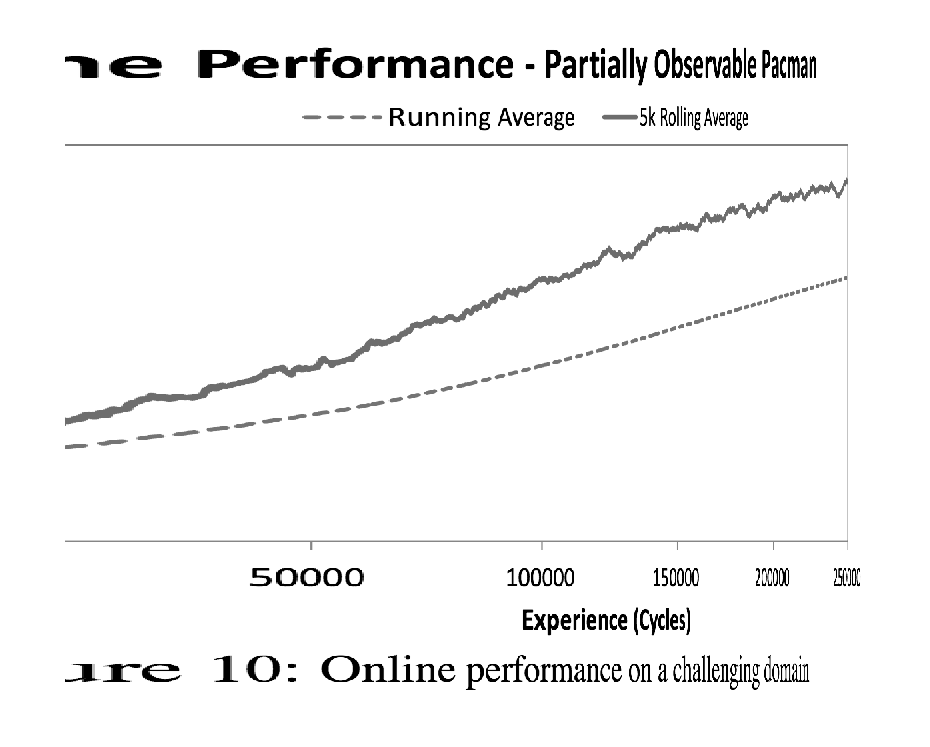
\includegraphics[width=\textwidth]{jvlg1002.png}
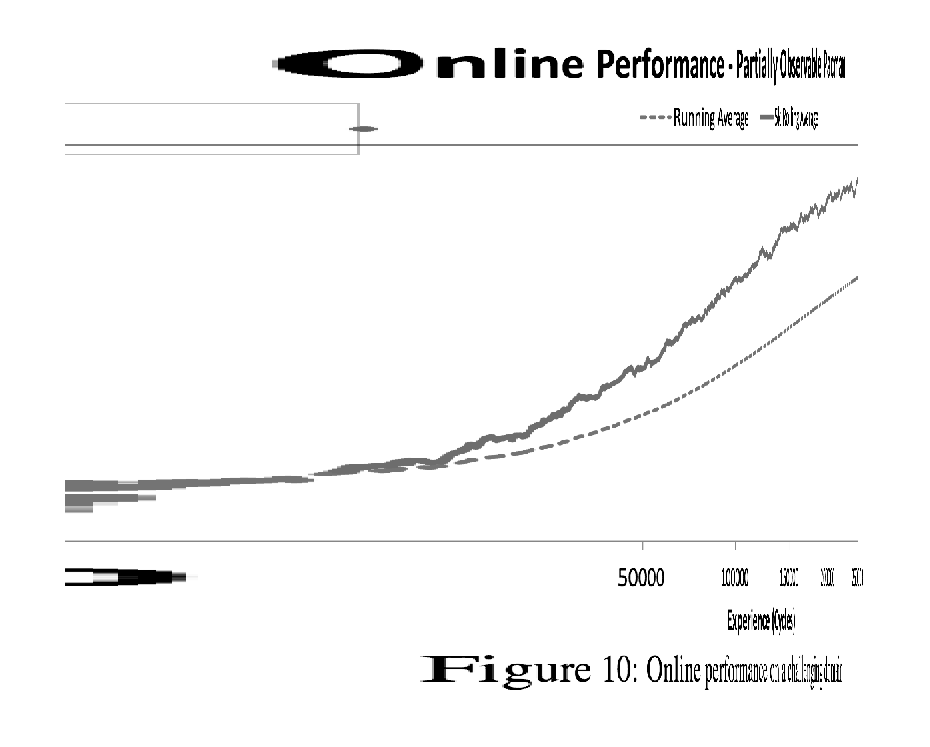
\includegraphics[width=\textwidth]{jvlg1005.png}
\caption{
Log-transformed image of plot from \cite{orig}\label{fig:jvl},
solid lines showing current performance.
}
\end{figure}

%\begin{figure}
%\begin{tikzpicture}[trim axis left]
%\begin{axis}[ \stdAOM , skip coords between index={0}{1},
%	each nth point = 20,
%	filter discard warning=false,
%	skip coords between index={10001}{999999}
%	]
%\one{sp2-p0-pacman.csv} \addlegendentry{E=0 D=1 H=4 R}
%\one{sp2-p1-pacman.csv} \addlegendentry{E=0 D=32 H=4 R}
%\one{sp2-p2-pacman.csv} \addlegendentry{E=0 D=1 H=16 R}
%\one{sp2-p3-pacman.csv} \addlegendentry{E=0 D=32 H=16 R}
%\one{sp1-p-pacman.csv} \addlegendentry{D=80 H=4 R}
%\one{sp2-p-pacman.csv} \addlegendentry{D=32 H=16 R}
%\end{axis}
%\end{tikzpicture}
%\cpt{\label{fig:pm1} PacMan}
%
%\end{figure}

Finally, a visual inspection of the
\verb|txt| files with ASCII graphics
suggested that our agents
with low horizon did learn to play pacman,
in particular avoiding running into walls,
evade ghosts, and eat food if nearby.
To see for oneself, check 
\begin{verbatim}
logs/pm-*.txt
\end{verbatim}
e.g.
\begin{verbatim}
logs/pm-32-1-d.txt
\end{verbatim}
You can also ask us to program
a player to print the \verb|txt|
files with timing to make it
animated.

\section{Conclusion}

We were able to let the agent play all the games as specified,
in particular PacMan.

It remains to be an interesting problem how we can get the
agent to play deterministically on CoinFlip.
While easy to reason about, playing deterministically
is not necessarily the first thing to occur to a human either.

%A frequent notable phenomenon is that agents sometimes 
%learn to play with a strategy “taken exploration into consideration”,
%that is when exploration rates drops further the agent starts
%play worse. While it is not hard to imagine a model 
%has only gone through insufficient training may perform
%worse than random, it is not so obvious that it can be
%improved by mixing with random play.

Most importantly, especially in the maze-related games,
a simpler model seemed to be better, to the point of
using a search horizon of 1.
The size of tree, or memory capabilities, are not
monotonic to game performance either.
Directly giving the agent an accurate model 
does not necessarily result in the best performance.

In PacMan it seemed more important to be general
than to be accurate.
It is not hard to imagine that there could be very simple
strategies just to “survive” in a maze-like environment,
without actually learning an accurate model of the environment.
In real world, many organisms live with basic reflexes.

Moreover, the PacMan game, due to its partial observablity,
actually resembles a first-person shooter game \cite{fps},
though there are no first-person shooter game
as simple as PacMan, since it is a genre began
in the 1990s. For a human, this type of games can be
easily played “only with reflexes”, at 
least to a leisure level(i.e. 
not competing or pursuing a high score), while the game environment
is complex (modern FPS are huge in terms of storage
and even RAM usage).

At the opposite end are board games, which in our
tests required us to use larger search
horizons.
In this games an accurate model of the world
also gave clear advantage.
Except for professionals and
aficionados, playing Chess is usually more exhausting than
playing Call of Duty, 
while programming a playble Chess game is a negligible
effort than developing (as it far surpasses programming) Call of Duty,
or even the first version of DOOM, the same to the computational
resource needed to run the games.






\bibliographystyle{unsrt}
\bibliography{ref}

\end{flushleft}
\end{document}
